\documentclass{beamer}
\usetheme{Madrid}
\usecolortheme{default}

\title[Traffic Speed Prediction]
{Traffic Speed Prediction Near the\\University of Toronto}

\subtitle{Group XX: [Group Name]}

\author[Group XX: Group Name]
{Member 1\inst{1} \and Member 2\inst{1} \and Member 3\inst{1}}

\institute[ ]
{
  \inst{1}%
  Dept.\ of ECE, University of Toronto
}

\date[IntroML]
{Introduction to Machine Learning -- Winter 2026}

\logo{
\includegraphics[height=0.8cm]{logo_uoft}}

\definecolor{uoftblue}{RGB}{6,41,88}
\setbeamercolor{titlelike}{bg=uoftblue}
\setbeamerfont{title}{series=\bfseries}

\usepackage{booktabs}
\usepackage{graphicx}

\begin{document}

\frame{\titlepage}


% ── SLIDE 1: Problem Definition ──────────────────────────────
\begin{frame}
\frametitle{Problem Definition}

\textbf{Goal:} Predict average traffic speed (km/h) on city streets near U\,of\,T St.\ George campus at 15-minute intervals.

\bigskip
\textbf{Why this matters:}
\begin{itemize}\setlength\itemsep{4pt}
  \item Urban congestion costs Toronto billions annually
  \item Existing sensors give real-time data but limited forecasting
  \item 15-min ahead predictions enable proactive routing and planning
  \item Patterns vary by road segment, time of day, weather, and season
\end{itemize}

\bigskip
\textbf{Approach:}
\begin{itemize}\setlength\itemsep{4pt}
  \item Progressive model improvement: XGBoost $\rightarrow$ neural network
  \item 47 experiments via autonomous ``autoresearch'' loop
  \item Evaluation: MAE, RMSE, R$^2$ on chronological test split
\end{itemize}
\end{frame}


% ── SLIDE 2: Data ────────────────────────────────────────────
\begin{frame}
\frametitle{Data Overview}

\begin{columns}[T]
\begin{column}{0.47\textwidth}
\textbf{Traffic Speed Data}
\begin{itemize}\setlength\itemsep{3pt}
  \item Toronto Open Data Portal
  \item 2.1M records (2020--2025)
  \item 14 speed bins $\rightarrow$ weighted avg
  \item 15-min intervals
  \item 1{,}947 segments after filtering
\end{itemize}
\end{column}
\begin{column}{0.47\textwidth}
\textbf{Weather Data}
\begin{itemize}\setlength\itemsep{3pt}
  \item Environment Canada (Stn.\ 6158359)
  \item 54K hourly records (2020--2026)
  \item Temp, wind, precip, visibility
  \item Humidity
  \item Rain / snow / fog flags
\end{itemize}
\end{column}
\end{columns}

\bigskip
\textbf{Merged dataset:} 1.58M rows, 49 engineered features.

\medskip
\textbf{Split:} 70\% train / 10\% validation / 20\% test --- strictly chronological, no shuffling.
\end{frame}


% ── SLIDE 3: Feature Engineering ─────────────────────────────
\begin{frame}
\frametitle{Feature Engineering}

\textbf{49 features} across four categories:

\bigskip
{\small
\begin{tabular}{@{}llll@{}}
\toprule
\textbf{Temporal} & \textbf{Weather} & \textbf{Lag \& Rolling} & \textbf{Historical} \\
\midrule
Hour, DOW, month   & Temperature   & Speed dev lags (1--16) & Avg spd / seg / hr / DOW \\
Sin/cos encoding   & Wind, precip  & Volume dev lags        & Speed deviation          \\
Rush-hour flags    & Visibility    & Rolling mean \& std    & Lagged interactions      \\
Weekend flag       & Rain/snow/fog & Raw speed rolling      &                          \\
\bottomrule
\end{tabular}
}

\bigskip
\textbf{Key design decisions:}
\begin{itemize}\setlength\itemsep{3pt}
  \item Lag features use \emph{deviation} (not raw speed) to avoid data leakage
  \item Rolling windows shifted by 1--2 steps to prevent lookahead
  \item Segments with $<$72 hours of data removed (noise reduction)
\end{itemize}
\end{frame}


% ── SLIDE 4: Model Progression ───────────────────────────────
\begin{frame}
\frametitle{Model Progression}

47 experiments run via autoresearch loop (modify $\rightarrow$ train $\rightarrow$ eval $\rightarrow$ keep/revert):

\bigskip
\centering
{\small
\begin{tabular}{@{}clcl@{}}
\toprule
\textbf{\#} & \textbf{Model} & \textbf{Test MAE} & \textbf{Key change} \\
\midrule
1 & XGBoost baseline     & 2.246 & Default hyperparameters \\
2 & + feature engineering & 2.082 & Rush-hour flags, lag 12/16, data filter \\
3 & + MAE loss objective  & 2.018 & Align training loss with eval metric \\
4 & PyTorch MLP           & 1.931 & Switch to neural network on GPU \\
5 & ResNet MLP            & 1.848 & Add residual skip connections \\
\textbf{6} & \textbf{Final model} & \textbf{1.825} & \textbf{+ 2025 data, SiLU, deviation target} \\
\bottomrule
\end{tabular}
}

\bigskip
\flushleft
\textbf{Total improvement:} 18.7\% MAE reduction (2.246 $\rightarrow$ 1.825).

\medskip
28 experiments kept, 19 discarded. Inspired by \texttt{karpathy/autoresearch}.
\end{frame}


% ── SLIDE 5: Architecture ────────────────────────────────────
\begin{frame}
\frametitle{Final Model Architecture}

\begin{columns}[T]
\begin{column}{0.45\textwidth}
\centering
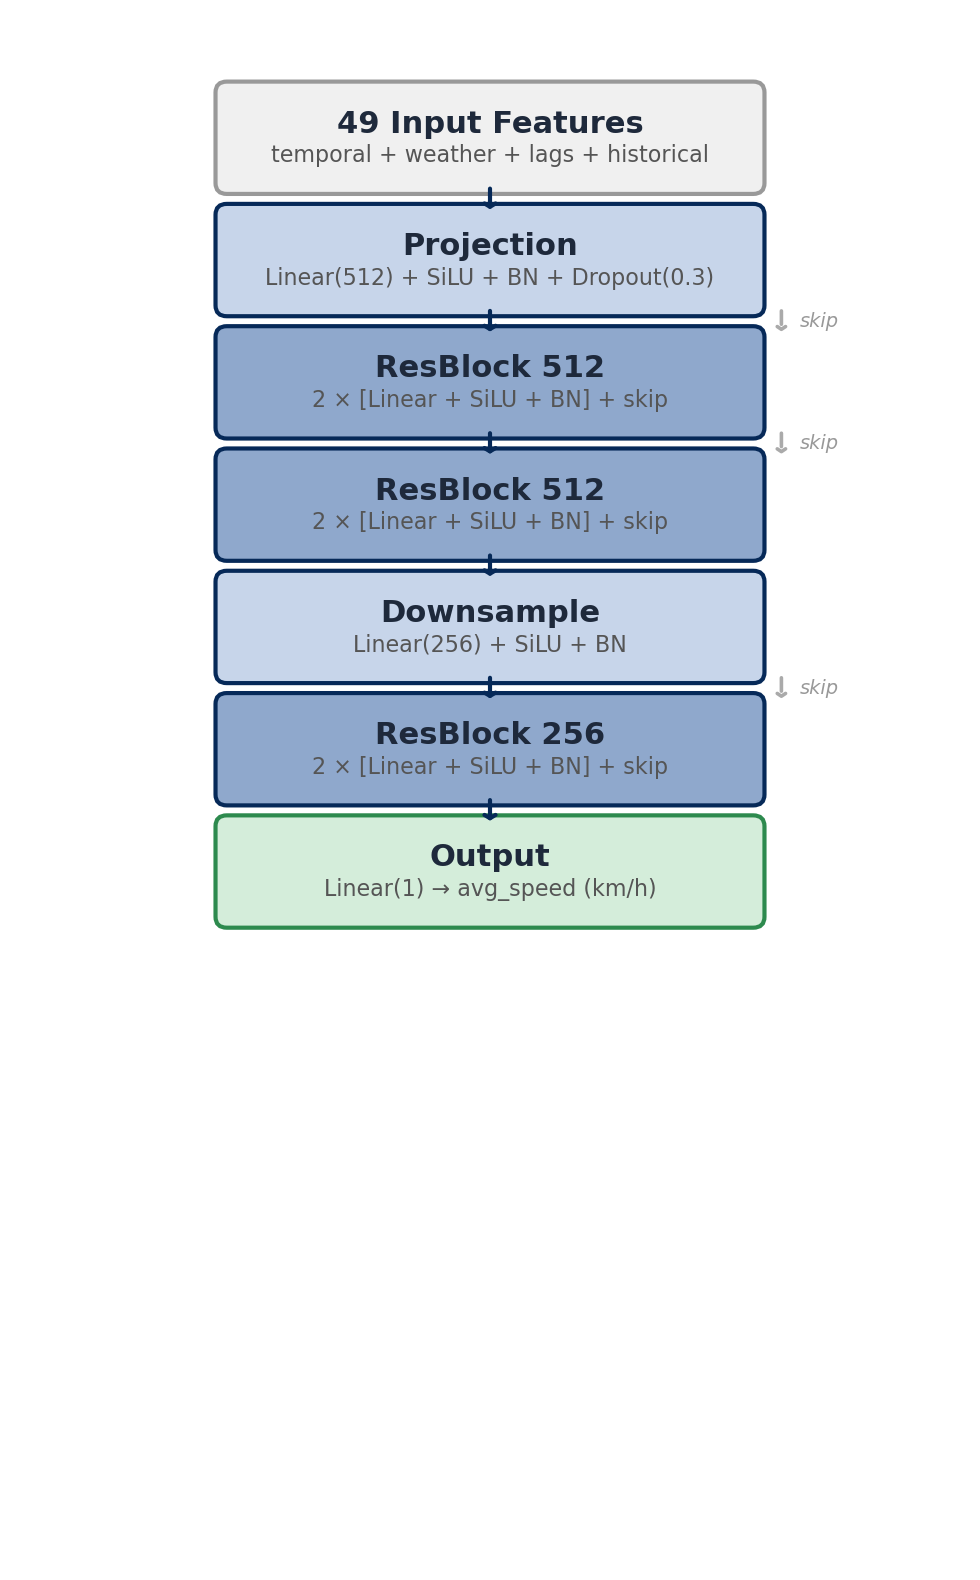
\includegraphics[height=7.2cm]{arch_diagram.png}
\end{column}

\begin{column}{0.52\textwidth}
\textbf{Training configuration:}

\medskip
{\small
\begin{tabular}{@{}ll@{}}
\toprule
Optimizer  & AdamW (lr=1e-3, wd=1e-4) \\
Scheduler  & ReduceLROnPlateau \\
Loss       & L1 (MAE) \\
Batch size & 4096 \\
Early stop & patience 20 epochs \\
Grad clip  & max\_norm 1.0 \\
\midrule
GPU        & RTX 5090 (32 GB) \\
Train time & $\sim$50 seconds \\
\bottomrule
\end{tabular}
}

\bigskip
\textbf{Target:} \texttt{speed\_deviation}

\smallskip
{\small
Predict deviation from historical average speed per segment/hour/DOW. Add back the mean at inference to recover km/h.
}

\bigskip
\textbf{Why deviation?}
\begin{itemize}\setlength\itemsep{2pt}
  \item Centers target near zero
  \item Historical mean handles per-location baseline
\end{itemize}
\end{column}
\end{columns}
\end{frame}


% ── SLIDE 6: Results ─────────────────────────────────────────
\begin{frame}
\frametitle{Results}

\centering
{\small
\begin{tabular}{@{}lcccc@{}}
\toprule
\textbf{Model} & \textbf{MAE} & \textbf{RMSE} & \textbf{R$^2$} & \textbf{Improvement} \\
\midrule
XGBoost Baseline & 2.246 & 3.418 & 0.891 & --- \\
XGBoost Tuned    & 2.018 & 3.220 & 0.904 & 10.2\% \\
Simple MLP       & 1.931 & 3.120 & 0.910 & 14.0\% \\
ResNet MLP       & 1.848 & 3.091 & 0.911 & 17.7\% \\
\textbf{Final (best)} & \textbf{1.825} & \textbf{3.055} & \textbf{0.917} & \textbf{18.7\%} \\
\bottomrule
\end{tabular}
}

\bigskip
\begin{columns}[T]
\begin{column}{0.47\textwidth}
\textbf{What worked:}
\begin{itemize}\setlength\itemsep{2pt}
  \item MAE loss alignment
  \item Filtering noisy segments
  \item Residual connections
  \item SiLU activation
  \item Deviation target
  \item More data (+370K rows from 2025)
\end{itemize}
\end{column}
\begin{column}{0.47\textwidth}
\textbf{What didn't work:}
\begin{itemize}\setlength\itemsep{2pt}
  \item Entity embeddings
  \item CatBoost GPU
  \item OneCycleLR scheduler
  \item GELU, SmoothL1, LayerNorm
  \item XGBoost + MLP ensemble
\end{itemize}
\end{column}
\end{columns}
\end{frame}


\end{document}
